\documentclass[dvisvgm,border=2pt]{standalone}
% Shared by every figure. Two colours only: black becomes the text colour of
% whatever theme the app is in, and `accent` becomes the brand — see
% scripts/build-figures.mjs. Everything else is done with opacity.
\usepackage{amsmath}
\usepackage{amssymb}
\usepackage{tikz}
\usepackage{pgfplots}
\pgfplotsset{compat=1.18}
\usetikzlibrary{arrows.meta,positioning,calc,backgrounds,fit,patterns.meta}
\definecolor{accent}{RGB}{255,0,255}
\pgfplotsset{
  every axis/.append style={
    axis lines=left,
    axis line style={draw opacity=0.35},
    tick style={draw opacity=0.35},
    tick label style={font=\scriptsize,opacity=0.7},
    label style={font=\scriptsize,opacity=0.7},
    legend style={draw=none,fill=none,font=\scriptsize},
    every axis plot/.append style={line width=0.7pt},
  },
}
\tikzset{
  every picture/.style={font=\scriptsize},
  faint/.style={opacity=0.3},
  quiet/.style={opacity=0.55},
  box/.style={draw,opacity=0.35,rounded corners=2pt,inner sep=4pt},
  hot/.style={accent},
}

\begin{document}
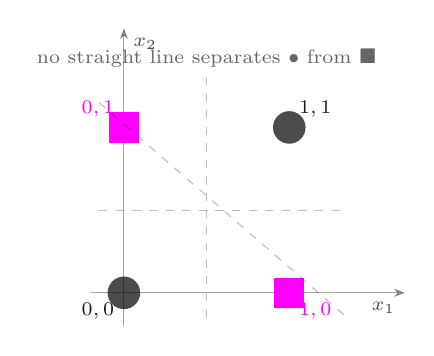
\begin{tikzpicture}[scale=2.1]
  \draw[opacity=0.35,-{Stealth[length=4pt]}] (-0.2,0) -- (1.7,0) node[below left,opacity=0.7]{$x_1$};
  \draw[opacity=0.35,-{Stealth[length=4pt]}] (0,-0.2) -- (0,1.6) node[below right,opacity=0.7]{$x_2$};
  \fill[opacity=0.7] (0,0) circle (2.8pt) node[below left,opacity=0.9]{$0,0$};
  \fill[opacity=0.7] (1,1) circle (2.8pt) node[above right,opacity=0.9]{$1,1$};
  \fill[accent] (0,1) ++(-2.6pt,-2.6pt) rectangle ++(5.2pt,5.2pt);
  \node[above left,accent] at (0,1) {$0,1$};
  \fill[accent] (1,0) ++(-2.6pt,-2.6pt) rectangle ++(5.2pt,5.2pt);
  \node[below right,accent] at (1,0) {$1,0$};
  \draw[opacity=0.25,dashed] (-0.15,0.5) -- (1.35,0.5);
  \draw[opacity=0.25,dashed] (0.5,-0.15) -- (0.5,1.35);
  \draw[opacity=0.25,dashed] (-0.15,1.15) -- (1.35,-0.15);
  \node[opacity=0.6,align=center] at (0.5,1.42) {no straight line separates \(\bullet\) from \(\blacksquare\)};
\end{tikzpicture}
\end{document}
